\documentclass[a4paper,11pt]{article}

\newcommand{\authorinfo}{Paul Bienkowski, Konstantin Kobs}
\newcommand{\titleinfo}{Robotics Assignment \#02}

% PREAMBLE ===============================================================

%\usepackage[german,ngerman]{babel}
\usepackage[utf8]{inputenc}
\usepackage[T1]{fontenc}
\usepackage[top=1.3in, bottom=1in, left=1.0in, right=0.6in]{geometry}
\usepackage{lmodern}
\usepackage{amssymb}
\usepackage{mathtools}
\usepackage{amsmath}
\usepackage{enumerate}
\usepackage{pgfplots}
\usepackage{breqn}
\usepackage{tikz}
\usepackage{fancyhdr}
\usepackage{multicol}
\usepackage{gensymb}
\allowdisplaybreaks

\usetikzlibrary{calc}
\usetikzlibrary{patterns}

\author{\authorinfo}
\title{\titleinfo}
\date{\today}

\pagestyle{fancy}
\fancyhf{}
\fancyhead[L]{\authorinfo}
\fancyhead[R]{\titleinfo}
\fancyfoot[C]{\thepage}

\begin{document}
\maketitle
\begin {enumerate}
\item[\textbf{Task 2.1.}]

    \begin{enumerate}
        \item[1)] The manipulator transformation is a series of multiple rotational $Rot_z(\theta_i)$ and translational $Trans_{x_i}(a_i)$ transformations. That means, $^0T_3 = {^0A_1} {^1A_2} {^2A_3}$ is given by
        	\begin{align*}
        		^0A_1 &= Rot_z(\theta_1) \cdot Trans_{x_1}(a_1)\\
        		^1A_2 &= Rot_z(\theta_2) \cdot Trans_{x_2}(a_2)\\
        		^2A_3 &= Rot_z(\theta_3) \cdot Trans_{x_3}(a_3)
        	\end{align*}
        	where $Rot_z(\theta_i) = \begin{bmatrix}
        		C_i & -S_i & 0 & 0\\
        		S_i & C_i & 0 & 0\\
        		0 & 0 & 1 & 0\\
        		0 & 0 & 0 & 1
        	\end{bmatrix}$
        	and
        	$Trans_{x_i}(a_i) = \begin{bmatrix}
        		1 & 0 & 0 & a_i\\
        		0 & 1 & 0 & 0\\
        		0 & 0 & 1 & 0\\
        		0 & 0 & 0 & 1
        	\end{bmatrix}$.
        	
        	With this in mind, we can calculate the partial homogeneous transformations:
	        	$${^0A_1} = \begin{bmatrix} C_1 & -S_1 & 0 & C_1a_1\\ S_1 & C_1 & 0 & S_1a_1\\ 0 & 0 & 1 & 0\\ 0 & 0 & 0 & 1 \end{bmatrix} \quad
	        	{^1A_2} = \begin{bmatrix} C_2 & -S_2 & 0 & C_2a_2\\ S_2 & C_2 & 0 & S_2a_2\\ 0 & 0 & 1 & 0\\ 0 & 0 & 0 & 1 \end{bmatrix}\quad
	        	{^2A_3} = \begin{bmatrix} C_3 & -S_3 & 0 & C_3a_3\\ S_3 & C_3 & 0 & S_3a_3\\ 0 & 0 & 1 & 0\\ 0 & 0 & 0 & 1 \end{bmatrix}$$
   
    For intermediate results, we first calculate $^0T_2 = {^0A_1}{^1A_2}$ and then $^0T_3 = {^0T_2}{^2A_3}$.
    \begin{align*}
    	^0T_2 &= \begin{bmatrix} C_1 & -S_1 & 0 & C_1a_1\\ S_1 & C_1 & 0 & S_1a_1\\ 0 & 0 & 1 & 0\\ 0 & 0 & 0 & 1 \end{bmatrix} \begin{bmatrix} C_2 & -S_2 & 0 & C_2a_2\\ S_2 & C_2 & 0 & S_2a_2\\ 0 & 0 & 1 & 0\\ 0 & 0 & 0 & 1 \end{bmatrix}\\
    	&= \begin{bmatrix} C_1C_2 - S_1S_2 & -C_1S_2 - S_1C_2 & 0 & C_1C_2a_2 -S_1S_2a_2 + C_1a_1\\ S_1C_2 + C_1S_2 & -S_1S_2 + C_1C_2 & 0 & S_1C_2a_2 + C_1S_2a_2 + S_1a_1\\ 0 & 0 & 1 & 0\\ 0 & 0 & 0 & 1 \end{bmatrix}\\
    	&= \begin{bmatrix} C_{1+2} & -S_{1+2} & 0 & C_{1+2}a_2 + C_1a_1\\ S_{1+2} & C_{1+2} & 0 & S_{1+2}a_2 + S_1a_1\\ 0 & 0 & 1 & 0\\ 0 & 0 & 0 & 1 \end{bmatrix}\\
    	^0T_3 &= \begin{bmatrix} C_{1+2} & -S_{1+2} & 0 & C_{1+2}a_2 + C_1a_1\\ S_{1+2} & C_{1+2} & 0 & S_{1+2}a_2 + S_1a_1\\ 0 & 0 & 1 & 0\\ 0 & 0 & 0 & 1 \end{bmatrix} \begin{bmatrix} C_3 & -S_3 & 0 & C_3a_3\\ S_3 & C_3 & 0 & S_3a_3\\ 0 & 0 & 1 & 0\\ 0 & 0 & 0 & 1 \end{bmatrix}\\
    	&= \begin{bmatrix} C_{1+2}C_3 - S_{1+2}S_3 & -C_{1+2}S_3 - S_{1+2}C_3 & 0 & C_{1+2}C_3a_3 - S_{1+2}S_3a_3 + C_{1+2}a_2+C_1a_1\\ S_{1+2}C_3 + C_{1+2}S_3 & -S_{1+2}S_3+C_{1+2}C_3 & 0 & S_{1+2}C_3a_3 + C_{1+2}S_3a_3 + S_{1+2}a_2 + S_1a_1\\ 0 & 0 & 1 & 0\\ 0 & 0 & 0 & 1 \end{bmatrix}\\
    	&= \begin{bmatrix} C_{1+2+3} & -S_{1+2+3} & 0 & C_{1+2+3}a_3 + C_{1+2}a_2+C_1a_1\\ S_{1+2+3} & C_{1+2+3} & 0 & S_{1+2+3}a_3 + S_{1+2}a_2 + S_1a_1\\ 0 & 0 & 1 & 0\\ 0 & 0 & 0 & 1 \end{bmatrix}
    \end{align*}
	
	Because the relation $\theta_1 + \theta_2 + \theta_3 = 180\degree$ is given, we can simplify the results. For $\cos(180\degree) = -1$ and $\sin(180\degree) = 0$:
		$${^0T_3} = \begin{bmatrix}
			-1 & 0 & 0 & -a_3 + C_{1+2}a_2+C_1a_1\\
			0 & -1 & 0 & S_{1+2}a_2 + S_1a_1\\
			0 & 0 & 1 & 0\\
			0 & 0 & 0 & 1
		\end{bmatrix}$$
	Furthermore, $\cos(\alpha) = -\cos(180\degree - \alpha)$ and $\sin(\alpha) = \sin(180\degree - \alpha)$ for $\alpha \in [0\degree, 180\degree]$. These facts result in the given transformation matrix:
		$${^0T_3} = \begin{bmatrix}
			-1 & 0 & 0 & C_1a_1 - C_{3}a_2 - a_3\\
			0 & -1 & 0 & S_1a_1 + S_{3}a_2\\
			0 & 0 & 1 & 0\\
			0 & 0 & 0 & 1
		\end{bmatrix}$$
        \item[2)] To rotate around $x_0$, we need to use Euler angles and append the rotation transformation matrix to the left side of ${^0T_3}$, because we need to rotate the manipulator before the other transformation can be started.
        \begin{align*}
        	{^0T_3}' &= Rot_{x_0}(\theta_0) \cdot {^0T_3}\\
        	&= \begin{bmatrix}
			1 & 0 & 0 & 0\\
			0 & C_0 & -S_0 & 0\\
			0 & S_0 & C_0 & 0\\
			0 & 0 & 0 & 1
		\end{bmatrix} \begin{bmatrix}
			-1 & 0 & 0 & C_1a_1 - C_{3}a_2 - a_3\\
			0 & -1 & 0 & S_1a_1 + S_{3}a_2\\
			0 & 0 & 1 & 0\\
			0 & 0 & 0 & 1
		\end{bmatrix}\\
			&= \begin{bmatrix}
			-1 & 0 & 0 & C_1a_1 - C_{3}a_2 - a_3\\
			0 & -C_0 & -S_0 & C_0S_1a_1 + C_0S_{3}a_2\\
			0 & -S_0 & C_0 & S_0S_1a_1 + S_0S_3a_2\\
			0 & 0 & 0 & 1
		\end{bmatrix}
        \end{align*}
        
        For the second rotation around $x_3$ by $\theta_4$, we append the rotation matrix to the right side of ${^0T_3}$.
        \begin{align*}
        	{^0T_3}'' &= {^0T_3} \cdot Rot_{x_3}(\theta_4)\\
        	&= \begin{bmatrix}
			-1 & 0 & 0 & C_1a_1 - C_{3}a_2 - a_3\\
			0 & -1 & 0 & S_1a_1 + S_{3}a_2\\
			0 & 0 & 1 & 0\\
			0 & 0 & 0 & 1
		\end{bmatrix} \begin{bmatrix}
			1 & 0 & 0 & 0\\
			0 & C_4 & -S_4 & 0\\
			0 & S_4 & C_4 & 0\\
			0 & 0 & 0 & 1
		\end{bmatrix}\\
			&= \begin{bmatrix}
			-1 & 0 & 0 & C_1a_1 - C_{3}a_2 - a_3\\
			0 & -C_4 & S_4 & S_1a_1+S_3a_2\\
			0 & S_4 & C_4 & 0\\
			0 & 0 & 0 & 1
		\end{bmatrix}
        \end{align*}
        
    \end{enumerate}

\item[\textbf{Task 2.2.}]


\item[\textbf{Task 2.3.}] The coordinate frames are specified via the figure \ref{fig:2.3}. In this drawing, every z-axis points towards the viewer, in order to complete a right-handes coordinate system.
	
	\begin{figure}[!ht]
	\center
		\raisebox{-0.5\height}{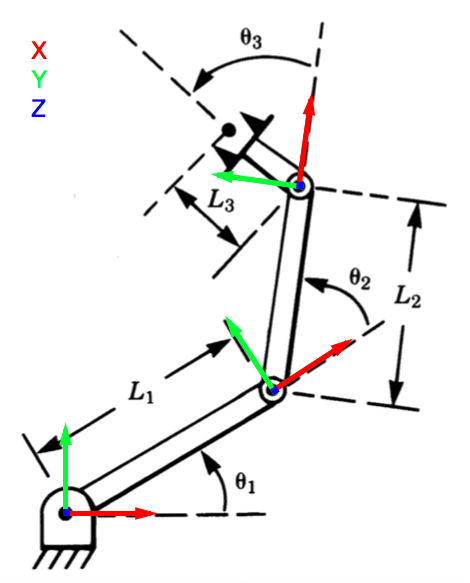
\includegraphics[height=9cm]{2-3.png}}
	\qquad
	\begin{tabular}{|c|c|c|c|c|}
		\hline 
		Link i & $\theta_i$ & $\alpha_{i-1}$ & $a_{i-1}$ & $d_i$ \\ 
		\hline 
		1 & $\theta_1$ & $0\degree$ & $L_1$ & 0 \\ 
		\hline 
		2 & $\theta_2$ & $0\degree$ & $L_2$ & 0 \\ 
		\hline 
		3 & $\theta_3$ & $0\degree$ & $L_3$ & 0 \\
		\hline 
	\end{tabular}
	\caption{The specified coordinate frames and the DH parameters of 2.3}
	\label{fig:2.3}
	\end{figure}

	
    
\item[\textbf{Task 2.4.}]

    \begin{enumerate}
        \item[1)] The manipulator shown in the figure follows the Denavit-Hartenberg-convention. Every z-axis is given by the axis of rotation of its joint. Every x-axis shows in the directions of the common normal of both z-axes, or better in the direction of the shortest connection between both z-axes, since there are no common normals for parallel z-axes. Every y-axis and every rotation direction is then given by the fact, that we want to have a right handed coordinate system.
        \item[2)] The homogeneous transformation $^{Base}T_{Tool}$ is given by concatenation of the partial transformations from one frame to the next:
        $${^{Base}T_{Tool}} = {^0T_1}{^1T_2}{^2T_3}{^3T_4}$$
        We determine the partial transformation matrices as follows and convert milimeters to meters to avoid big numbers:
        \begin{align*}
        	{^0T_1} &= Trans_{(0,0,877mm)} \cdot Rot_{z_0}(\theta_1) \cdot Trans_{(425mm,0,0)} \cdot Rot_{x_0}(\pi)\\
        	&= \begin{pmatrix}
        		1 & 0 & 0 & 0\\
        		0 & 1 & 0 & 0\\
        		0 & 0 & 1 & 0.877\\
        		0 & 0 & 0 & 1\\
        	\end{pmatrix}        	
        	\begin{pmatrix}
        		\cos(\theta_1) & -\sin(\theta_1) & 0 & 0\\
        		\sin(\theta_1) & \cos(\theta_1) & 0 & 0\\
        		0 & 0 & 1 & 0\\
        		0 & 0 & 0 & 1\\
        	\end{pmatrix}\\
        	&\qquad\qquad \begin{pmatrix}
        		1 & 0 & 0 & 0.425\\
        		0 & 1 & 0 & 0\\
        		0 & 0 & 1 & 0\\
        		0 & 0 & 0 & 1\\
        	\end{pmatrix}
        	\begin{pmatrix}
        	    1 & 0 & 0 & 0\\
        		0 & \cos(\pi) & -\sin(\pi) & 0\\
        		0 & \sin(\pi) & \cos(\pi) & 0\\
        		0 & 0 & 0 & 1\\
        	\end{pmatrix}\\
        	&= \begin{pmatrix}
        		\cos(\theta_1) & -\sin(\theta_1) & 0 & 0\\
        		\sin(\theta_1) & \cos(\theta_1) & 0 & 0\\
        		0 & 0 & 1 & 0.877\\
        		0 & 0 & 0 & 1\\
        	\end{pmatrix}
        	\begin{pmatrix}
        		1 & 0 & 0 & 0.425\\
        		0 & 1 & 0 & 0\\
        		0 & 0 & 1 & 0\\
        		0 & 0 & 0 & 1\\
        	\end{pmatrix}\\
        	&\qquad\qquad \begin{pmatrix}
        	    1 & 0 & 0 & 0\\
        		0 & -1 & 0 & 0\\
        		0 & 0 & -1 & 0\\
        		0 & 0 & 0 & 1\\
        	\end{pmatrix}\\
        	&= \begin{pmatrix}
        		\cos(\theta_1) & -\sin(\theta_1) & 0 & 0.425 \cdot \cos(\theta_1)\\
        		\sin(\theta_1) & \cos(\theta_1) & 0 & 0.425 \cdot \sin(\theta_1)\\
        		0 & 0 & 1 & 0.877\\
        		0 & 0 & 0 & 1\\
        	\end{pmatrix}
        	\begin{pmatrix}
        	    1 & 0 & 0 & 0\\
        		0 & -1 & 0 & 0\\
        		0 & 0 & -1 & 0\\
        		0 & 0 & 0 & 1\\
        	\end{pmatrix}\\
        	&= \begin{pmatrix}
        		\cos(\theta_1) & \sin(\theta_1) & 0 & 0.425 \cdot \cos(\theta_1)\\
        		\sin(\theta_1) & -\cos(\theta_1) & 0 & 0.425 \cdot \sin(\theta_1)\\
        		0 & 0 & -1 & 0.877\\
        		0 & 0 & 0 & 1\\
        	\end{pmatrix}\\
% End of Calculation 1
        	{^1T_2} &= Rot_{z_1}(\theta_2) \cdot Trans_{(375mm,0,0)}\\
        	&= \begin{pmatrix}
        		\cos(\theta_2) & -\sin(\theta_2) & 0 & 0\\
        		\sin(\theta_2) & \cos(\theta_2) & 0 & 0\\
        		0 & 0 & 1 & 0\\
        		0 & 0 & 0 & 1\\
        	\end{pmatrix}
        	\begin{pmatrix}
        		1 & 0 & 0 & 0.375\\
        		0 & 1 & 0 & 0\\
        		0 & 0 & 1 & 0\\
        		0 & 0 & 0 & 1\\
        	\end{pmatrix}\\
        	&= \begin{pmatrix}
        		\cos(\theta_2) & -\sin(\theta_2) & 0 & 0.375 \cdot \cos(\theta_2)\\
        		\sin(\theta_2) & \cos(\theta_2) & 0 & 0.375 \cdot \sin(\theta_2)\\
        		0 & 0 & 1 & 0\\
        		0 & 0 & 0 & 1\\
        	\end{pmatrix}\\
% End of Calculation 2
        	{^2T_3} &= Trans_{(0,0,d_3)}\\
        	&= \begin{pmatrix}
        		1 & 0 & 0 & 0\\
        		0 & 1 & 0 & 0\\
        		0 & 0 & 1 & d_3\\
        		0 & 0 & 0 & 1\\
        	\end{pmatrix}\\
% End of Calculation 3
        	{^3T_4} &= Trans_{(0,0,200mm)} \cdot Rot_{z_3}(\pi/2 + \theta_4)\\
        	&= \begin{pmatrix}
        		1 & 0 & 0 & 0\\
        		0 & 1 & 0 & 0\\
        		0 & 0 & 1 & 0.2\\
        		0 & 0 & 0 & 1\\
        	\end{pmatrix}
        	\begin{pmatrix}
        		\cos(\pi/2 + \theta_4) & -\sin(\pi/2 + \theta_4) & 0 & 0\\
        		\sin(\pi/2 + \theta_4) & \cos(\pi/2 + \theta_4) & 0 & 0\\
        		0 & 0 & 1 & 0\\
        		0 & 0 & 0 & 1\\
        	\end{pmatrix}\\
        	&= \begin{pmatrix}
        		\cos(\pi/2 + \theta_4) & -\sin(\pi/2 + \theta_4) & 0 & 0\\
        		\sin(\pi/2 + \theta_4) & \cos(\pi/2 + \theta_4) & 0 & 0\\
        		0 & 0 & 1 & 0.2\\
        		0 & 0 & 0 & 1\\
        	\end{pmatrix}\\
        \end{align*}
        Now we can compute the final transformation matrix:
        \begin{align*}
        	{^{Base}T_{Tool}} &= {^0T_1}{^1T_2}{^2T_3}{^3T_4}\\
        	&= \begin{pmatrix}
        		C_1C_2 + S_1S_2 & -S_2C_1 + S_1C_2 & 0 & 0.375C_1C_2 + 0.375S_1S_2 + 0.425C_1\\
        		S_1C_2-C_1S_2 & -S_1S_2-C_1C_2 & 0 & 0.375S_1C_2-0.375C_1S_2+0.425S_1\\
        		0 & 0 & -1 & 0.877\\
        		0 & 0 & 0 & 1\\
        	\end{pmatrix} {^2T_3}{^3T_4}\\
        	&= \begin{pmatrix}
        		C_1C_2 + S_1S_2 & -S_2C_1 + S_1C_2 & 0 & 0.375C_1C_2 + 0.375S_1S_2 + 0.425C_1\\
        		S_1C_2-C_1S_2 & -S_1S_2-C_1C_2 & 0 & 0.375S_1C_2-0.375C_1S_2+0.425S_1\\
        		0 & 0 & -1 & -d_3 + 0.877\\
        		0 & 0 & 0 & 1\\
        	\end{pmatrix} {^3T_4}\\
        	&= \begin{pmatrix}
        		n_x & o_x & a_x & p_x\\
        		n_y & o_y & a_y & p_y\\
        		n_z & o_z & a_z & p_z\\
        		0 & 0 & 0 & 1\\
        	\end{pmatrix}\\
        	\text{with:}&\\
        	n_x &= (C_1C_2 + S_1S_2)\cos(\pi/2 + \theta_4) + (-S_2C_1 + S_1C_2)\sin(\pi/2 + \theta_4)\\
			n_y &= (S_1C_2-C_1S_2)\cos(\pi/2 + \theta_4) + (-S_1S_2 - C_1C_2)\sin(\pi/2 + \theta_4)\\
			n_z &= 0\\
			o_x &= -(C_1C_2 + S_1S_2)\sin(\pi/2 + \theta_4) + (-S_2C_1 + S_1C_2)\cos(\pi/2 + \theta_4) = n_y\\
			o_y &= -(S_1C_2-C_1S_2)\sin(\pi/2 + \theta_4) + (-S_1S_2 - C_1C_2)\cos(\pi/2 + \theta_4) = -n_x\\
			o_z &= 0\\
			a_x &= 0\\
			a_y &= 0\\
			a_z &= -1\\
			p_x &= 0.375C_1C_2 + 0.375S_1S_2 + 0.425C_1\\
			p_y &= 0.375S_1C_2-0.375C_1S_2+0.425S_1\\
			p_z &= -0.2 - d_3 + 0.877\\
        \end{align*}
        where $C_i = \cos(\theta_i)$ and $S_i = \sin(\theta_i)$.
        
        \item[3)] Before we can calculate the result, we need to insert the variables into ${^{Base}T_{Tool}}$. \textbf{Note:} Since we work with \textit{meters} and not with \textit{mm} we need to convert $120$ to $0.12$. Overall, this leads to:
        $${^{Base}T_{Tool}} \approx \begin{pmatrix}
        	-0.7071 & -0.9659 & 0 & 0.2035\\
        	-0.9659 & 0.7071 & 0 & 0.6627\\
        	0 & 0 & -1 & 0.557\\
        	0 & 0 & 0 & 1 \\
        \end{pmatrix}$$
        Assuming the origin of the base frame is the origin of the world coordinate system (at $(0,0,0)$), we can calculate the coordinates of the tool center point as follows:
        \begin{align*}
        	{^{Base}T_{Tool}} \cdot \begin{pmatrix}
        		0\\0\\0\\1
        	\end{pmatrix} &\approx \begin{pmatrix}
        	-0.7071 & -0.9659 & 0 & 0.2035\\
        	-0.9659 & 0.7071 & 0 & 0.6627\\
        	0 & 0 & -1 & 0.557\\
        	0 & 0 & 0 & 1 \\
        \end{pmatrix} \cdot \begin{pmatrix}
        		0\\0\\0\\1
        	\end{pmatrix}\\
        &\approx \begin{pmatrix}
        		0.2035\\0.6627\\0.557\\1
        	\end{pmatrix}
        \end{align*}
        The tool center point is at the point $(203.5, 662.7, 557)$ of the base coordinate system.
        
        
    \end{enumerate}

\end {enumerate}
\end{document}
